\documentclass[12pt]{article}

\usepackage[utf8]{inputenc}
\usepackage{latexsym,amsfonts,amssymb,amsthm,amsmath,graphicx}


\setlength{\parindent}{0in}
\setlength{\oddsidemargin}{0in}
\setlength{\textwidth}{6.5in}
\setlength{\textheight}{8.8in}
\setlength{\topmargin}{0in}
\setlength{\headheight}{18pt}



\title{ASTR 218 Lecture Notes: Lecture 10}
\author{Bayu Wilson}
\date{October 14, 2019}

\begin{document}

\maketitle

\vspace{0.5in}


\section{The Need for Bayesian Statistics}
Prior to Bayesianism, statistics generally consisted of \textbf{classical hypothesis testing}, a framework often encountered by undergraduates. For example, when combining errors there is a simple formula which is derived by assuming that most probabilities are Gaussian distributed:
\begin{align*}
      x_1 & \sim  N(\mu_1,\sigma_1^2) \\
      x_2 & \sim  N(\mu_2,\sigma_2^2) \\
      x_1+x_2 &\sim  N(\mu_1+\mu_2,\sigma_1^2+\sigma_2^2) \\
\end{align*}

Frequentism is, generally, a set of statistical techniques which arose at a time when experimental science was concerned with arbitrarily repeatable experiments, and when theoreticians needed something they could calculate with. It is concerned with probabilities of events occurring in the long run, works out the probability of some particular dataset occurring under some model and often makes a simplifying Gaussian approximation to this probability for practical reasons. 

Gaussian approximations are used for two reasons:
\begin{enumerate}
  \item The Central Limit Theorem says everything measured with a large enough sample size is approximately Gaussian (or Normal) distributed
  \item Ease of calculation. Gaussians are easy to integrate.
\end{enumerate}

Bayesian statistics was able to advance because computational power increased. With computers, statisticians can explore arbitrary distributions that aren't Gaussian, and model experiments in complicated and interesting ways.

Note that in practice we often still approximate likelihood functions as Gaussian, but it is important to know that, especially far from the peak, this is rarely a good model. Generally the far tails of a distribution are larger than a Gaussian predicts (see Figure~\ref{fig:gaussian_noise_plot}).

\begin{figure}[ht]
%\includegraphics[scale=0.42]{paper_mf.pdf}
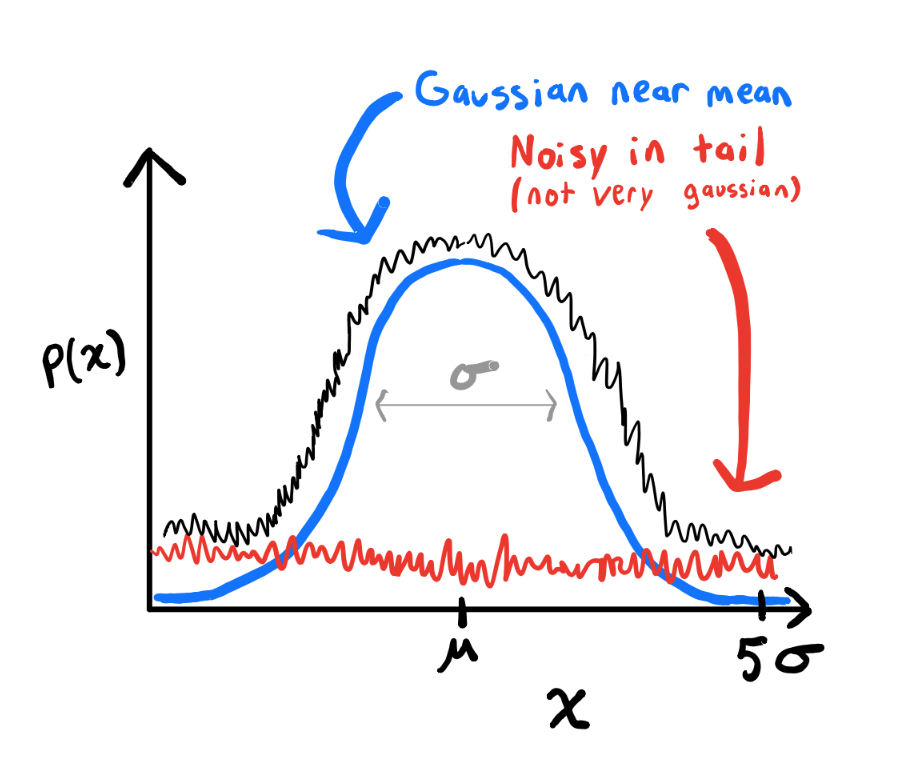
\includegraphics[scale=0.75]{gaussian_noise_plot.png}
\centering
\caption{An cartoon example of most probability distributions in real life. Near the mean (within 1$\sigma$) one can approximate the distribution (black line) as Gaussian (blue line). However, in the tail ($\sim 5\sigma$) the distribution is often fatter (red line).} \label{fig:gaussian_noise_plot}
\end{figure}

\newpage
\subsection{Bayes' Theorem}
Bayes' Theorem can be written as the following:
\begin{equation}
    P(M|D) = \frac{P(D|M)P(M)}{P(D)}
\end{equation}
In some sense this is just a restatement of the definition of conditional probability:
\begin{equation}
    P(A|B)P(B) = P(B|A)P(A)
\end{equation}
but we are writing down now our amount of belief in a model, not the concrete occurrence of physical events.

\subsection{Notation \& Definitions}
\begin{itemize}
  \item M is a model (an essential part of Bayesianism)
  \item D is experimental data
    \item $P(M|D)$ is the probability of the model given data, the posterior. This is the thing that you want. Note we compute a probability but we do not give a decision threshold as to whether the model is true.
    \item $P(D|M)$ is the probability of the data given the model. It is also called the likelihood.
    \item $P(M)$ is the prior: it doesn't depend on data. This is the prior belief in the absence of data. It can model earlier experiments of your own inherent theoretical prejudices. It is in principle subjective and you may validly choose different priors. However, as shown in Figure~\ref{fig:prior_plot}, as long as you choose a prior which is much wider than the posterior, its effect will be mild. If you have a prior that is not wider than the posterior, you need a better experiment!
    \item $P(D)$ is the total probability of the data. This is a strange quantity, naively impossible to compute. Instead we cheat, and find it by using the normalization of probabilities: $\sum_i P(M_i|D)=1$. Note that this asserts that we have considered all possible models, which is never really the case.
\end{itemize}

\begin{figure}[ht]
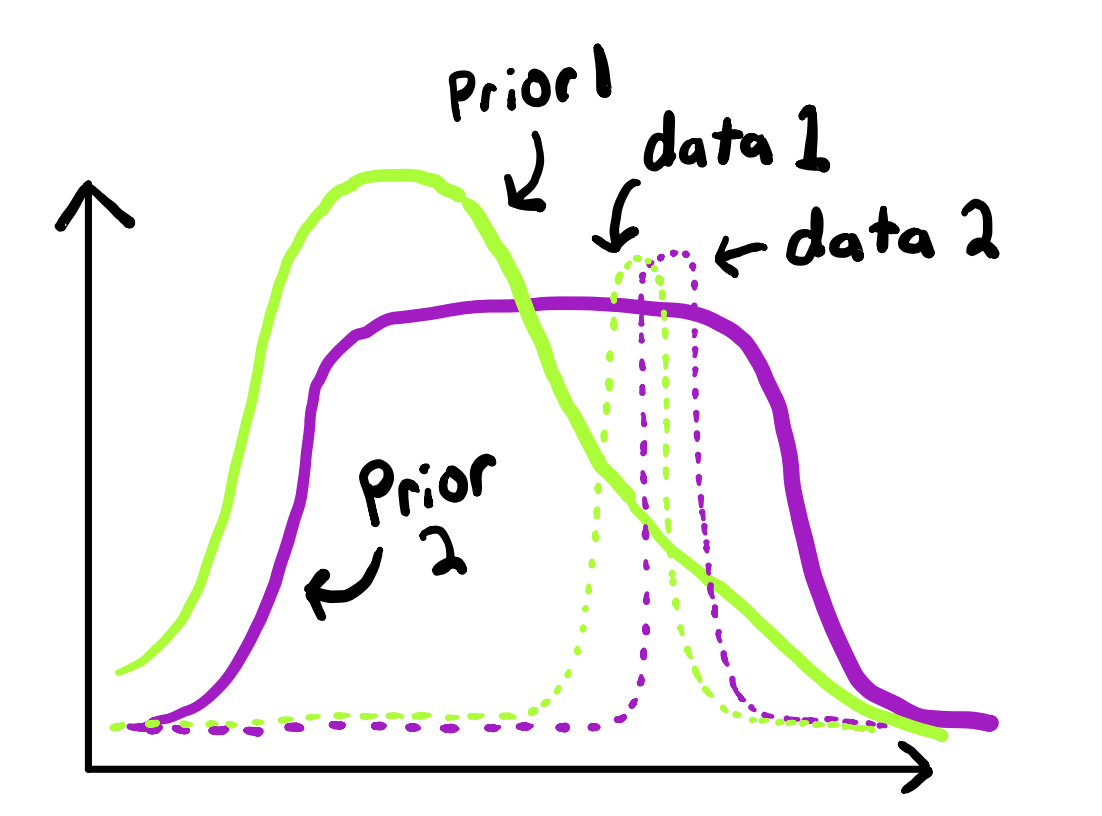
\includegraphics[scale=0.75]{prior_plot.png}
\centering
\caption{An cartoon example of how one's choice of prior can affect the posterior probability (data). Generally, the prior should always be \textbf{broader} than the data.} \label{fig:prior_plot}
\end{figure}


\end{document}
